\documentclass[12pt,a4paper,notitlepage]{article}
\usepackage[utf8]{inputenc}
\usepackage[a4paper,textwidth=17cm, top=2cm, bottom=3.5cm]{geometry}
\usepackage[T1]{fontenc}
\usepackage[
    backend=biber,
    style=numeric,
    natbib=true,
    url=true, 
    doi=true,
    eprint=false
    ]{biblatex}
\addbibresource{directions.bib}
\usepackage{amssymb,amsmath}
\usepackage{listings}
\usepackage{eurosym}
\usepackage{wasysym}
\usepackage{amsthm}
\usepackage{tabularx}
\usepackage{multirow}
\usepackage{multicol}
\usepackage{tikz}

\usetikzlibrary{arrows}
\usetikzlibrary{backgrounds}
\usetikzlibrary{calc}
\usetikzlibrary{decorations.markings}
\usetikzlibrary{decorations.pathreplacing}
\usetikzlibrary{fit}
\usetikzlibrary{patterns}  
\usetikzlibrary{positioning}
\usetikzlibrary{shapes}

\usepackage{hyperref}
\usepackage{tabularx}
\usepackage{commath}
\usepackage{graphicx,color}
\usepackage{subcaption}
\usepackage{float}
\usepackage{footmisc}
\usepackage{array}
\usepackage[underline=false]{pgf-umlsd}
\usetikzlibrary{calc}
%\usepackage[pdftex]{graphicx,color}
%\usepackage{epstopdf}

\newcommand{\foonote}[1]{\footnote{#1}}
\newcommand{\degree}{\ensuremath{^\circ}}
\newcolumntype{P}[1]{>{\centering\arraybackslash}p{#1}}

\author{Sebastian Götte {\texttt<secureusb@jaseg.net>} @Mori lab, Waseda University}
\title{Research directions in secure USB devices}
\date{December 12 2018}
\begin{document}
\maketitle

\section{Introduction}
\subsection{Problem definition}
A computer's USB interface is hard to secure. Though overall security is quite good today, the USB interface has not
received enough attention. In particular HIDs are a problem, as they are naturally very highly privileged.
Off-the-shelf USB HID attack tools exist. In particular from a security point of view extremely bad ideas such as
WebUSB\cite{misc01} are set to increase this already large attack surface even further.

\subsection{Contributions}
This work includes three key contributions. First, it demonstrates a practical implementation of a complete,
backwards-compatible secure USB system using QubesOS and a single new piece of security hardware.  Second, it shows a
novel interactive user-friendly cryptographic handshaking scheme based on out-of-band communication. Third, it shows and
proposes some techniques for the design of general secure protocols that are not limited to USB alone.

\section{The state of the art in mitigation}
Several ways to secure the USB interface have been proposed that can be broadly categorized as follows.
\begin{itemize}
    \item USB firewalls are software or hardware that protects the host from requests deemed invalid similar to a network firewall\cite{tian01,angel01,kang01,bates01,loe01}.
    \item USB device authentication uses some sort of user feedback or public key infrastructure to authenticate the device when it connects\cite{usb01,griscioli01,wang01,he01}.
    \item USB bus encryption encrypts the raw USB payloads to ward off eavesdroppers\cite{neugschwandtner01,weinstein01}.
    \item For wireless protocols, every conceivable pairing model has been tried. However, not many have been applied to
        USB\cite{arun01,uzun01,kobsa01,saxena01}.
    \item Compartmentalized systems such as QubesOS separate vulnerable components with large attack surface such as the USB device drivers into VMs to not inhibit exploitation but mitigate its consequences.
\end{itemize}

\begin{table}
    \setlength{\extrarowheight}{5pt}
    \begin{tabular}{l|P{10mm}|P{15mm}|P{15mm}|P{15mm}|P{17mm}|P{25mm}|}
                                &\multicolumn{3}{c|}{\bfseries Attacks}                                             & \multicolumn{2}{c|}{\bfseries Eavesdropping} & \multirow{2}{25mm}{\centering\bfseries Backwards\newline compatible} \\\cline{2-6}
                                & \bfseries HID     &\bfseries Host\newline exploit &\bfseries Device\newline exploit&\bfseries Bus-level &\bfseries Physical layer    & \\\hline
        Firewalls               & $\bigcirc$        & $\triangle$                   & $\times$                      & $\triangle$   & $\times$          & $\bigcirc$ \\
        Device authentication   & $\bigcirc$        & $\times$                      & $\times$                      & $\triangle$   & $\times$          & $\times$ \\
        Bus encryption          & $\triangle$       & $\times$                      & $\times$                      & $\bigcirc$    & $\bigcirc$        & $\times$ \\
        Plain QubesOS setup\footnotemark 
                                & $\triangle$       & $\triangle$                   & $\triangle$                   & $\triangle$   & $\times$          & $\bigcirc$ \\
        Our work                & $\bigcirc$        & $\bigcirc$                    & $\bigcirc$                    & $\bigcirc$    & $\bigcirc$        & $\bigcirc$
    \end{tabular}
    \caption{Comparison of approaches to USB security}
    \label{approach_comparison}
\end{table}
\footnotetext{Requires separate USB host controller for HIDs}

We compare these approaches w.r.t. several attacks in \ref{approach_comparison}. Overall we found that QubesOS is the
only advance towards securing this interface that is both \emph{practical} and \emph{effective}. Other approaches have
not been successful so far. A likely reason for this is large market inertia and necessary backwards-compatibility.

QubesOS approaches the problem by running a separate VM with the USB host controllers mapped through via IOMMU. This VM
runs a linux kernel with a small set of white-listed USB device drivers (HID and mass storage device) and a USB-over-IP
backend. A set of Qubes services pass through any HID input arriving inside this VM into dom0, and coordinate exporting
USB mass storage devices as Xen block devices. Any other USB devices can be passed-through to other VMs through
USB-over-IP-over-QubesRPC, a Xen vChan-based inter-VM communication system.

QubesOS is still lacking in that it's compartmentalization becomes essentially useless when it is used with a USB HID
keyboard that does not have its own dedicated PCIe USB host controller, as any normal desktop and most recent laptop
computers. The issue here is that USB HID is neither authenticated nor encrypted, and the untrusted USB VM sits in the
middle of this data stream, which thus allows it trivial privilege escalation via keystroke injection.

\subsection{Usage scenarios}

Today USB's level security is still adequate for most everyday users. In general, attacks against USB either require
special malicious hardware or require re-flashing of existing peripherals with custom malicious firmware. Today's
low-level cybercrime targeting everyday users is still focused on much easier tasks such as stealing passwords through
phishing, installing cryptolocker malware by means of malicious email attachments and extracting sensitive user data
with malicious browser addons. Fortunately, we have not yet entered an age where average computer users need to worry
about the type of attack this work defends against. Still, it can be expected that with the general increase of overall
computer security, eventually attackers will have to graduate to more advanced means--and since at this time the
landscape of effective defenses against USB attacks is very sparse, your author considers it important to explore the
avenues to effective defence ealier rather than later in order to be prepared for evolving attacks.

Despite the banality of everyday cybersecurity described above, there already are some people and organizations who face
advanced attacks including USB attacks. Due to their exceedingly simple execution, USB HID attacks are a very attractive
way to perform targeted attacks. For this reason, specialized USB attack hardware is already available commercially at
low cost. For users facing targeted attacks like this, SecureHID might already provide practical benefits.

The users most at risk of targeted attacks are those either working with highly sensitive data or working with highly
privileged access. The former group would include people such as journalists working with their sources and politicians
working with confidential information. The latter group would include law enforcement officials, often being endowed
with wide-ranging electronic access to databases and other confidential information. Further, system administrators and
computer programmers are often provided highly privileged access to critical systems for software deployment using
systems such as Ansible or uploading software packages into software repositories such as PyPI.

In all of these scenarios there are many users with very poweful adversaries. In case of a software developer or systems
administrator that would be competing companies or foreign intelligence agencies trying to gain access to internal
networks to steal confidential information. In case of a journalist that would be whoever they are writing about and
here the most interesting articles might come with the most powerful enemies. Finally, a security researcher would by
nature of their work, out of academic interest specifically be looking for the most dangerous targets they could find.

Some users might be able to reduce their attack surface to USB attacks by reducing their use of untrusted USB devices,
but in many everyday scenarios such as those described above this is not an option. A security researcher needs to
connect to untrusted devices in order to analyze them, and using a second, isolated machine for this is very
inconvenient. A journalist or politician will frequently have to read USB flash drives with documents for their work,
and again simply solving the problem by air-gapping is an effective but impractical mitigation. In all of these cases,
SecureHID would be an effective mitigation.

\section{Approach}
\subsection{System overview}
The goal of SecureHID is to enable the first reasonably secure system using both HID and arbitrary untrusted devices on
the same USB host controller, based on QubesOS. SecureHID consists of a USB HID encryption box to be put between
keyboard and computer and a piece of software run inside QubesOS. After initial pairing with the host software, the
encryption box will encrypt and sign any USB HID input arriving from the keyboard and forward the encrypted data to the
host. The host software running outside the untrusted USB VM will receive the encrypted and signed data from the
untrusted USB VM, verify and decrypt it, and inject the received HID input events into Qubes's input event handling
system.

A schematic diagram of a system employing SecureHID is shown in figure \ref{diagram_with}. Two major points that can be
seen here are that first, SecureHID requires no specialized hardware on either end and transparently plugs into the
existing USB stack. Second, a SecureHID-protected setup has two well-defined security boundaries, one inside the
SecureHID device between host and device side, and one in the host operating system between USB driver VM and
hypervisor.

These security boundaries allow a clean separation of a SecureHID setup into untrusted and trusted domains and greatly
simpliefies reasoning about overall system security.  Communication across these security boundaries is limited to the
simple SecureHID protocol. We describe the design of the SecureHID protocol in section \ref{prot_desc} and elaborate
its security properties in section \ref{prot_ver}. The security of the protocol's core components has been formally
verified in the past and the protocol has been kept simple enough to allow exhaustive verification and testing.

\begin{figure}[H]
    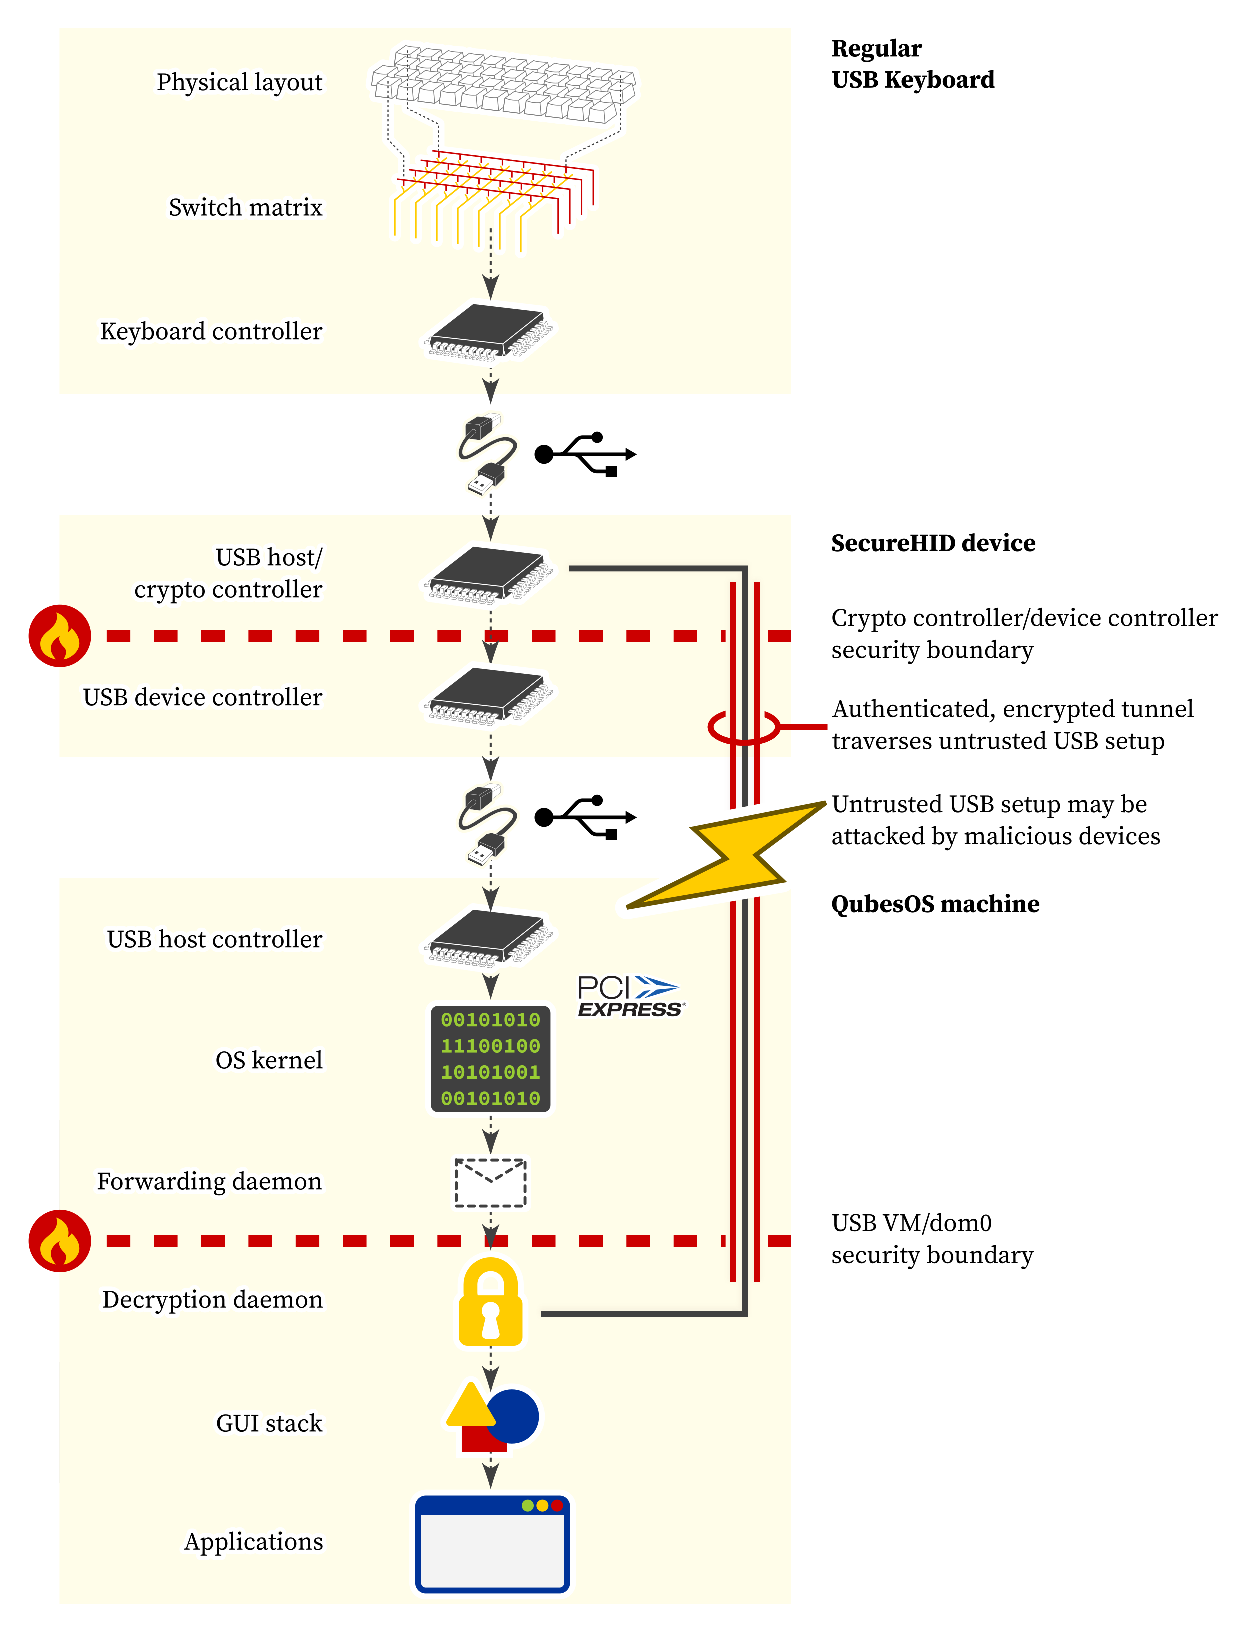
\includegraphics[scale=0.8]{system_diagram_with_secureusb.eps}
    \caption{Diagram of a SecureHID-protected system}
    \label{diagram_with}
\end{figure}

\subsection{Audio and other sensitive USB devices}
This system is sufficient to secure any USB setup, especially unmodified desktop PCs or laptops where a USB host
controller is shared between both HIDs and other devices. Attack surface is reduced such that a \emph{full compromise}
of the system becomes unlikely, since plain HID is no longer supported. The remaining attack surface consists only of a
\emph{compromise of the USB VM}. This attack surface is small enough that other sensitive devices such as USB audio
devices can safely be connected. A compromise of the USB driver VM no longer gives full system access, but at best
allows listening in on the microphone. Since a compromised USB VM does not have network access, such an attack will be
mostly harmless in most scenarios. Additionally, the most likely attacking devices would be custom hardware or a
smartphone. Custom hardware can easily be outfitted with a microphone, essentially turning it into a bug irrespective of
USB functionality, and smartphones already have microphones by definition.

A practical mitigation to this issue would be to simply connect microphones either to a PCIe-based sound card as in most
laptops, or to simply unplug the microphone when not used.

\subsection{USB physical-level and bus-level attacks}
Since sensitive HIDs are isolated from other USB devices effectively on a separate bus, bus-level attacks such as
\textcite{neugschwandtner01} are entirely prevented. Even much scarier physical attacks on USB such as \textcite{su01}
are prevented given an adequate hardware implementation, which fortunately is no too complicated.

\section{Cryptographic design}

\subsection{Protocol description}
\label{prot_desc}
The basic protocol consists of two stages: \textsc{pairing} and \textsc{data}. When the device powers up, it enters
\textsc{pairing} state. When the host enumerates a new device, it enters \textsc{pairing} state. If any fatal
communication errors occur, both host and device re-enter \textsc{pairing} state. To make the implementation robust
against host software crashing, devices being unplugged etc. without opening it up to attacks, the host can request the
device to re-enter \textsc{pairing} state a limited number of times after powerup.

\textsc{pairing} state consists of a number of substates as set by \textcite{perrin01}. The device runs noise's
\textsc{XX} scheme, i.e. both host and device each contribute both one ephemeral key $e$ and one static key $s$ to the
handshake, and the public halves of the static keys are transmitted during handshake encrypted by the emphemeral keys.

The cryptographic primitives instantiated in the prototype are X25519 for the ECDH primitive, BLAKE2s as a hash and
ChaCha20-Poly1305 as AEAD for the data phase. ECDH instead of traditional DH was chosen for its small key size and fast
computation. Since no variant of RSA is used, key generation is fast. An ad-hoc prototype device-side random number
generator has been implemented based on BLAKE2s and the STM32's internal hardware RNG.

\begin{figure}
    \centering
    \begin{sequencediagram}
        \newinst{kbd}{Keyboard}
        \newinst[3]{dev}{SecureHID}
        \newinst[5]{host}{Host}

        \mess{host}{}{dev}
        \path (mess from) -- (mess to) node[midway, above] {\emph{COBS sync (null byte)}};
        \mess{host}{}{dev}
        \draw[->,>=angle 60] (mess from) -- (mess to) node[midway, above] {\textsc{Initiate Handshake}};

        \begin{sdblock}{Noise XX handshake}{}
            \mess{host}{}{dev}
            \path (mess from) -- (mess to) node[midway, above] {$\textsc{Handshake}, e$};
            \mess{dev}{}{host}
            \path (mess from) -- (mess to) node[midway, above] {$\textsc{Handshake}, e,ee,s,es$};
            \mess{host}{}{dev}
            \path (mess from) -- (mess to) node[midway, above] {$\textsc{Handshake}, s,se$};
        \end{sdblock}

        \begin{sdblock}{Pairing}{Triggered by user interaction after unsuccessful handshake}
            \mess{dev}{}{host}
            \draw[->,>=angle 60] (mess from) -- (mess to) node[midway, above] {\textsc{Pairing Start}};
            \stepcounter{seqlevel}

            \mess{kbd}{keystroke}{dev}
            \addtocounter{seqlevel}{-1}
            \mess{dev}{}{host}
            \path (mess from) -- (mess to) node[midway, above] {$\textsc{Pairing Input},E(\text{keystroke})$};
            \stepcounter{seqlevel}
            \mess{kbd}{}{dev}
            \addtocounter{seqlevel}{-1}
            \path (mess from) -- (mess to) node[midway, above] {keystroke};
            \path (mess from) -- (mess to) node[midway, above, yshift=5mm] {$\vdots$};
            \mess{dev}{}{host}
            \path (mess from) -- (mess to) node[midway, above] {$\textsc{Pairing Input},E(\text{keystroke})$};
            \path (mess from) -- (mess to) node[midway, above, yshift=5mm] {$\vdots$};
            \stepcounter{seqlevel}

            \mess{kbd}{}{dev}
            \addtocounter{seqlevel}{-1}
            \path (mess from) -- (mess to) node[midway, above] {\emph{enter}};
            \mess{dev}{}{host}
            \draw[->,>=angle 60] (mess from) -- (mess to) node[midway, above] {\textsc{Pairing Success}};
        \end{sdblock}

        \begin{sdblock}{Input passthrough}{Started after successful handshake or pairing}
            \mess{kbd}{keystroke}{dev}
            \path (mess from) -- (mess to) node[midway, below, yshift=-2mm] {$\vdots$};

            \addtocounter{seqlevel}{-1}
            \mess{dev}{}{host}
            \path (mess from) -- (mess to) node[midway, above] {$\textsc{Data},E(\text{keystroke})$};
            \path (mess from) -- (mess to) node[midway, below, yshift=-2mm] {$\vdots$};
            \stepcounter{seqlevel}
        \end{sdblock}
    \end{sequencediagram}
    \caption{A successful prototype protocol pairing}
    \label{protocol_diagram}
\end{figure}

A successful pairing looks like this:
\begin{enumerate}
\item \textbf{Handshake.} \textsc{device} is connected to \textsc{host}
\item \textsc{host} initiates pairing by sending \textsc{initiate handshake} to device
\item \textsc{device} and \textsc{host} follow noise state machine for the \textsc{XX} handshake. See figure
	\ref{crypto_diagram} for a complete flowchart of cryptographic operations during this handshake. The handshake and
	subsequent Noise protocol communication are specified in \textcite{perrin01} and their security properties are
	formally verified in \textcite{kobeissi01}. Section \ref{sec_prop} analyzes the implications of these security
	properties for this research.
\item After the handshake completes, both \textsc{device} and \textsc{host} have received each other's static public key
    $rs$ and established a shared secret connection key. At this point, the possibility of an MITM attacker having
	actively intercepted the handshake remains. At this point \textsc{device} and \textsc{host} will both notice they do
	not yet know each other's static keys. \textsc{host} will respond to this by showing the pairing GUI dialog.
	\textsc{deivce} will sound an alarm to indicate an untrusted connection to the user.
\item \textbf{Channel binding.} Both \textsc{device} and \textsc{host} calculate the \emph{handshake hash} as per noise
	spec\cite{perrin01}. This hash uniquely identifies this session and depends on both local and remote ephemeral and
	static keys $le, re, ls, rs$.  Both parties encode a 64-bit part of this hash into a sequence of english words by
	dictionary lookup. This sequence of words is called the \emph{fingerprint} of the connection.
\item \textsc{host} prompts the user to enter the \emph{fingerprint} into a keyboard connected to \textsc{device}. The
	user presses the physical pairing button on \textsc{device} to stop the alarm and start pairing. This step prevents
	an attacker from being able to cause the device to send unencrypted input without user interaction by starting
	pairing.
\item As the user enters the \emph{fingerprint}, \textsc{device} relays any input over the yet-unauthenticated encrypted
    noise channel to \textsc{host}. \textsc{host} displays the received user input in plain text in a regular input
    field in the pairing GUI. This display is only for user convenience and not relevant to the cryptographic handshake.
    A consequence of this is that a MITM could observe the \emph{fingerprint}\footnote{
        A MITM could also modify the fingerprint information sent from \textsc{device} to \textsc{host}. This would be
        very obvious to the user, since the fingerprint appearing on the \textsc{host} screen would differ from what she
        types.
    }. We show in section \ref{prot_ver} that this does not reduce the protocol's security.
\item When the user has completed entering the fingerprint, the device checks the calculated fingerprint against the
    entered data. If both match, the host is signalled \textsc{success} and \textsc{data} phase is entered. If they do
    not match, the host is signalled \textsc{failure}\footnote{
        Note that this means a MITM could intercept the \textsc{failure} message and forge a \textsc{success} message.
        This means both are just for user convenience \emph{absent} an attacker. If an attacker is present, she will be
        caught in the next pairing step.
    } and \textsc{pairing} state is re-entered unless the maximum number of tries since powerup has been exceeded.
    Failure is indicated to the user by \textsc{device} through a very annoying beep accompanied by angrily flashing
    LEDs.
\item \textbf{Data phase.} \textsc{host} asks the user for confirmation of pairing \emph{in case the device did not
	sound an alarm} by pressing a button on the GUI. When the user does this, the host enters \textsc{data} state and
	starts input passthrough.
\end{enumerate}

Roughly speaking, this protocol is secure given that the only way to MITM a (EC)DH key exchange is to perform two (EC)DH
key exchanges with both parties, then relay messages. Since both parties have different static keys, the resulting two
(EC)DH sessions will have different handshake hashes under the noise framework. The channel binding step reliably
detects this condition through an out-of-band transmission of the \textsc{host} handshake hash to \textsc{device}.

The only specialty here is that this OOB transmission is relayed back from \textsc{device} to \textsc{host} allowing the
MITM to intercept it. This is only done for user convenience absent a MITM and the result is discarded by \textsc{host}.
Since the handshake hash does as a hash does not leak any sensitive information about the keys used during the
handshake, it being exposed does not impact protocol security.

\subsection{Protocol verifictation}
\label{prot_ver}
\subsubsection{Noise security properties}
\label{sec_prop}
According to \textcite{perrin01} and proven by \textcite{kobeissi01} Noise's XX pattern provides strong forward-secrecy,
sender and receiver authentication and key compromise impersonation resistance. Strong forward secrecy means an attacker
can only decrypt messages by compromising the receivers private key and performing an active impersonation.

Strong forward secrecy rules out both physical and protocol-level eavesdropping attacks by malicious USB devices and
implies that an attacker can never decrypt past protocol sessions. An implication of the static key checks done on both
sides of the connection is that an attacker would need to compromise both host and device in order to remain undetected
for e.g. keylogging.  Compromising only one party the worst that can be done is impersonating the SecureHID device to
perform a classical HID attack. In this case, the attacker cannot read user input.  The user would notice this by
SecureHID indicating a not connected status and no input being accepted.
% FIXME possibly detect this by having session counter etc.?

To verify that these security properties extend to the overall SecureHID protocol it suffices to show the following
three properties.
\begin{enumerate}
\item The SecureHID implementation of Noise XX adheres to the Noise specification, i.e. the handshake is performed
	correctly. \label{adh0}
\item Both sides' static keys are verified. \label{adh1}
\item All sensitive data is encapsulated in Noise messages after the handshake has ended, and none is sent before.
	\label{adh2}
\end{enumerate}

\ref{adh0} has been validated by manual code review and cross-validation of our implementation against other Noise
implementations. % FIXME write more, do more here
\ref{adh1} has been validated by manual code review. %FIXME do simulation here
Since all sensitive data in our application is handled on the device in a single place (the USB HID request handling
routine), \ref{adh2} is easily validated by code review. USB HID reports are only transmitted either encrypted after the
handshake has been completed or in plain during pairing. Since the host will only inject reports into the input
subsystem that have been properly authenticated and encrypted (and not the unauthenticated reports sent during pairing),
the protocol is secure in this regard.
% FIXME only start pairing after button press

\subsubsection{Handshake hash non-secrecy}

To analyze the impact of disclosing the handshake hash to an adversary we must consider it's definition. The noise
protocol specification gives its definition, but does not % FIXME double-check this 
guarantee that it can be disclosed to an adversary without compromising security. Figure \ref{crypto_diagram} contains a
flowchart of the derivation of both initiator-transmit and initiator-receive symmetric encryption keys $k_{1,2}$ and the
handshake hash $h$ during the Noise handshake. The definitions of MixHash and MixKey according to the Noise protocol
specification are as follows.

\begin{align}
	\text{MixHash}(h,\text{input}) &= h' = H(h || \text{input})\\
	\text{MixKey}(ck, \text{input}) &= (ck', k_\text{temp}) = \text{HKDF}(ck, \text{input}, 2)\\
\end{align}

Noise's hash-based key derivation function (HKDF) is defined using the HMAC defined in RFC2104\cite{rfc2104}. The hash
function $H$ employed here depends on the cipher spec used, in this work it is BLAKE2s.
\begin{equation}
	\text{HMAC}(K, \text{input}) = H\left(\left(K \oplus opad\right)
		|| H\left(\left(K \oplus ipad\right) || \text{input} \right)\right)
\end{equation}

The HKDF is defined for two and three outputs as follows.
\begin{equation}
	\text{HKDF}(ck, \text{input}, n_\text{out}) =
		\left\{\begin{array}{ll}
			(q_0, q_1) &: n_\text{out} = 2\\
			(q_0, q_1, q_2) &: n_\text{out} = 3\\
		\end{array}\right.
\end{equation}

The outputs $q_i$ are derived from chained HMAC invocations. First, a temporary key $t'$ is derived from the chaining key $ck$
and the input data using the $HMAC$, then depending on $n_\text{out}$ the HMAC is chained twice or thrice to produce
$q_{\{0,1,2\}}$.
\begin{gather}
	t' = \text{HMAC}(ck, \text{input})\\
	\underbrace{\text{HMAC} \Bigl(t',
	\underbrace{\text{HMAC} \bigl(t',
	\underbrace{\text{HMAC} (t',
		   1_{16})}_{q_0}
		|| 2_{16}\bigr)}_{q_1}
		|| 3_{16}\Bigr)}_{q_2}
\end{gather}

Figure \ref{crypto_diagram} shows the two properties relevant to this protocol implementation's security:
\begin{enumerate}
\item Initiator and responder ephemeral and static keys are all mixed into the handshake hash at least once.\label{fp1}
\item Knowledge of the handshake hash does not yield any information on the symmetric AEAD keys $k_1$ and $k_2$.\label{fp2}
\end{enumerate}

\ref{fp1} is evident since $e_i$ and $e_r$ are mixed in directly and $s_i$ and $s_r$ are mixed in after encryption with
temporary encryption keys derived from $ck$ at the $s\rightarrow$ and $s\leftarrow$ steps
during the handshake.

We can see \ref{fp2} applies by following the derivation of $h$ backwards. If an attacker learned anything about $k1$ or
$k2$ during an attack by (also) observing $h$ that they did not learn before, we could construct an oracle allowing both
reversal of $H$ in the final invocation of $MixHash$ and breaking $E$ using this attacker. The attacker would have to
reverse $H$ at some point since $h = H(\hdots)$ in the final invocation of MixHash. The attacker would have to recover
the key of $E$ in at least one invocation since $s_i$ and $s_r$ are only mixed into $h$ after either being encrypted
using $E$ or being used after ECDH to generate a key for $E$. Since the result of ECDH on $e_i$ and $e_r$ is mixed into
$h$ in the $ee\leftarrow$ and following DecryptAndHash steps, $h$ is blinded to an attacker so that they cannot even
determine a given $k_1$ and $k_2$ match a given $h$ without compromising ECDH security.

This means that given the underlying primitives are secure, we do not leak any information on $k1$ or $k2$ by disclosing
$h$.

\begin{figure}[h!]
	\centering
	\tikzset{%
		h/.style = {->, very thick},
		ck/.style = {->, very thick},
		key/.style = {->},
		ki/.style = {key, color=red},
		kr/.style = {key, color=red},
		ke/.style = {dashed},
		ks/.style = {solid},
		phaselbl/.style = {font=\bfseries, anchor=west}
	}
    \begin{tikzpicture}[scale=0.8]
        \node(protoname) at (0, 0){\texttt{"Noise\_XX\_25519\_ChaChaPoly\_BLAKE2s"}};
        \node[draw,thick,below=1em of protoname] (inithash) {$H$};
		\node[below=2em of inithash, xshift= 6.5em] (ck){$ck$};
		\node[below=2em of inithash, xshift=-6.5em] (h){$h$};
		\coordinate (labelbase) at (-5,0);

        \draw[->] (protoname) -- (inithash);
		\draw[->] (inithash) -- ++(0,-2em) coordinate(im0) -| (ck);
		\draw[->] (im0) -| (h);
		
		\node[right=7em of ck] (ei){$\mathbf{e_i}$};
		\node[right=8.5em of ck] (er){$\mathbf{e_r}$};
		\node[right=10em of ck] (si){$\mathbf{s_i}$};
		\node[right=11.5em of ck] (sr){$\mathbf{s_r}$};

		\node[draw,thick,below=3em of h] (mix0){MixHash};
		\node[right=1em of mix0] (str0){\texttt{""}};
		\node[left] at (str0 -| labelbase) (lbl0){\parbox{10em}{\raggedleft No preamble,\\use empty string}};

		\draw[h] (h) -- (mix0);
		\draw[->] (str0) -- (mix0);
		
%---
		\node[draw,thick,below=2em of mix0] (mix1){MixHash};
		\node[left] at (mix1 -| labelbase) (tok0){$e\rightarrow $};
		\draw[h] (mix0) -- (mix1);
		\draw[ki,ke] (ei) |- (mix1);

		\node[draw,thick,below=2em of mix1] (mix2){MixHash};
		\node[right=1em of mix2] (str2){\texttt{""}};
		\node[left] at (str2 -| labelbase) (lbl2){\parbox{10em}{\raggedleft EncryptAndHash\\No payload and\\$k$ unset}};
		\draw[->] (str2) -- (mix2);
		\draw[h] (mix1) -- (mix2);

		\coordinate (a) at ($ (mix0) !0.5! (mix1) $);
		\coordinate (b0) at (a -| lbl0.south west);
		\draw[dashed] (b0) -- ($ (b0 -| sr) + (1em,0) $);
%---
		\node[draw,thick,below=4em of mix2] (mix3){MixHash};
		\node[left] at (mix3 -| labelbase) (tok3){$e\leftarrow $};
		\draw[h] (mix2) -- (mix3);
		\draw[kr,ke] (er) |- (mix3);

		\coordinate (sync4) at (mix3 -| ck);
		\node[draw,thick,below=2em of sync4] (kmix1){MixKey};
		\node[left] at (kmix1 -| labelbase) (tok4){$ee\leftarrow $};
		\node[draw,thick,right=1em of kmix1] (dh0){ECDH};
		\draw[ck] (ck) -- (kmix1);
		\draw[ki,ke] (ei) |- ($ (dh0.east) + (0,0.2em) $);
		\draw[kr,ke] (er) |- ($ (dh0.east) - (0,0.2em) $);
		\draw[->] (dh0) -- (kmix1);

		\coordinate (sync5) at (kmix1 -| h);
		\node[draw,thick,below=2em of sync5] (mix5){MixHash};
		\node[draw,thick,right=2em of mix5] (enc5){$E$};
		\node[left] at (mix5 -| labelbase) (lbl5){$s\leftarrow $};
		\draw[h] (mix3) -- (mix5);
		\draw[->] (enc5) -- (mix5);
		\draw[->] ($ (kmix1.west) - (2em,0) $) -| (enc5);
		\draw[kr,ks] (sr) |- (enc5);

		\coordinate (sync6) at (mix5 -| ck);
		\node[draw,thick,below=2em of sync6] (kmix6){MixKey};
		\node[left] at (kmix6 -| labelbase) (tok6){$es\leftarrow $};
		\node[draw,thick,right=1em of kmix6] (dh6){ECDH};
		\draw[ck] (kmix1) -- (kmix6);
		\draw[ki,ke] (ei) |- ($ (dh6.east) + (0,0.2em) $);
		\draw[kr,ks] (sr) |- ($ (dh6.east) - (0,0.2em) $);
		\draw[->] (dh6) -- (kmix6);

		\coordinate (sync7) at (kmix6 -| h);
		\node[draw,thick,below=2em of sync7] (mix7){MixHash};
		\node[draw,thick,right=2em of mix7] (enc7){$E$};
		\node[right=1em of enc7] (str7){\texttt{""}};
		\node[left] at (mix7 -| labelbase) (lbl7){\parbox{10em}{\raggedleft DecryptAndHash\\ No payload}};
		\draw[h] (mix5) -- (mix7);
		\draw[->] (enc7) -- (mix7);
		\draw[->] (kmix1.west) -- ++(-2em,0) |- ($ (enc5.south) !0.25! (enc7.north) $) -- (enc7);
		\draw[->] (str7) -- (enc7);

		\coordinate (a) at ($ (mix2) !0.5! (mix3) $);
		\coordinate (b1) at (a -| lbl2.south west);
		\draw[dashed] (b1) -- ($ (b1 -| sr) + (1em,0) $);
% ---
		\node[draw,thick,below=4em of mix7] (mix8){MixHash};
		\node[draw,thick,right=2em of mix8] (enc8){$E$};
		\node[left] at (mix8 -| labelbase) (lbl8){$s\rightarrow $};
		\draw[h] (mix7) -- (mix8);
		\draw[->] (enc8) -- (mix8);
		\draw[->] (kmix6.west) -- ++(-2em,0) |- ($ (enc7.south) !0.25! (enc8.north) $) -- (enc8);
		\draw[ki,ks] (si) |- (enc8);

		\coordinate (sync9) at (mix8 -| ck);
		\node[draw,thick,below=2em of sync9] (kmix9){MixKey};
		\node[left] at (kmix9 -| labelbase) (tok9){$se\rightarrow $};
		\node[draw,thick,right=1em of kmix9] (dh9){ECDH};
		\draw[ck] (kmix6) -- (kmix9);
		\draw[ki,ks] (si) |- ($ (dh9.east) - (0,0.2em) $);
		\draw[kr,ke] (er) |- ($ (dh9.east) + (0,0.2em) $);
		\draw[->] (dh9) -- (kmix9);

		\coordinate (sync10) at (kmix9 -| h);
		\node[draw,thick,below=2em of sync10] (mix10){MixHash};
		\node[draw,thick,right=2em of mix10] (enc10){$E$};
		\node[right=1em of enc10] (str10){\texttt{""}};
		\node[left] at (mix10 -| labelbase) (lbl10){\parbox{10em}{\raggedleft EncryptAndHash\\ No payload}};
		\draw[h] (mix8) -- (mix10);
		\draw[->] (enc10) -- (mix10);
		\draw[->] (kmix9.west) -| (enc10);
		\draw[->] (str10) -- (enc10);

		\coordinate (a) at ($ (mix7) !0.5! (mix8) $);
		\coordinate (b2) at (a -| lbl2.south west);
		\draw[dashed] (b2) -- ($ (b2 -| sr) + (1em,0) $);
% ---
		\coordinate (sync11) at (mix10 -| ck);
		\node[draw,thick,below=5em of sync11,xshift=-1em] (finkdf){HKDF};
		\node[below=2em of finkdf,xshift=-1em] (k1){$\mathbf{k_1}$};
		\node[below=2em of finkdf,xshift= 1em] (k2){$\mathbf{k_2}$};
		\node[left=1em of finkdf,yshift=2em] (str11){\texttt{""}};
		\draw[ck] (kmix9) -- (finkdf.north -| kmix9);
		\draw[ck] (k1 |- finkdf.south) -- (k1);
		\draw[ck] (k2 |- finkdf.south) -- (k2);
		\draw[->] (str11) -| ($ (finkdf.north) - (1em,0) $);

		\coordinate (sync11a) at (finkdf.south -| h);
		\node[below=2em of sync11a] (hout){$\mathbf{h}$};
		\draw[h] (mix10) -- (hout);

		\node[left] at (finkdf -| labelbase) (lbl13){\parbox{10em}{\raggedleft Split}};

		\coordinate (a) at ($ (mix10) !0.5! (finkdf) $);
		\coordinate (b3) at (a -| lbl10.south west);
		\draw[dashed] (b3) -- ($ (b3 -| sr) + (1em,0) $);
%---
		\node[phaselbl, rectangle] at ($ (b0) !0.5! (b0 |- protoname) $) (setup){setup};
		\node[phaselbl, circle] at ($ (b0) !0.5! (b1) $) (ph0){0};
		\node[phaselbl, circle] at ($ (b1) !0.5! (b2) $) (ph1){1};
		\node[phaselbl, circle] at ($ (b2) !0.5! (b3) $) (ph2){2};
		\node[phaselbl, rectangle] at ($ (b3) !0.5! (b3 |- hout) $) (fin){fin};

    \end{tikzpicture}
    \caption{Cryptographic flowchart of Noise XX handshake.}
    \label{crypto_diagram}
\end{figure}

\section{Hardware implementation}
% FIXME

\section{Evaluation}
% FIXME

\section{Conclusion}
% FIXME

%\section{PCB design renderings}
%\label{ch:renderings}

%\begin{figure}[H]
%    \centering
%    \begin{subfigure}[b]{0.8\textwidth}
%        \centering
%        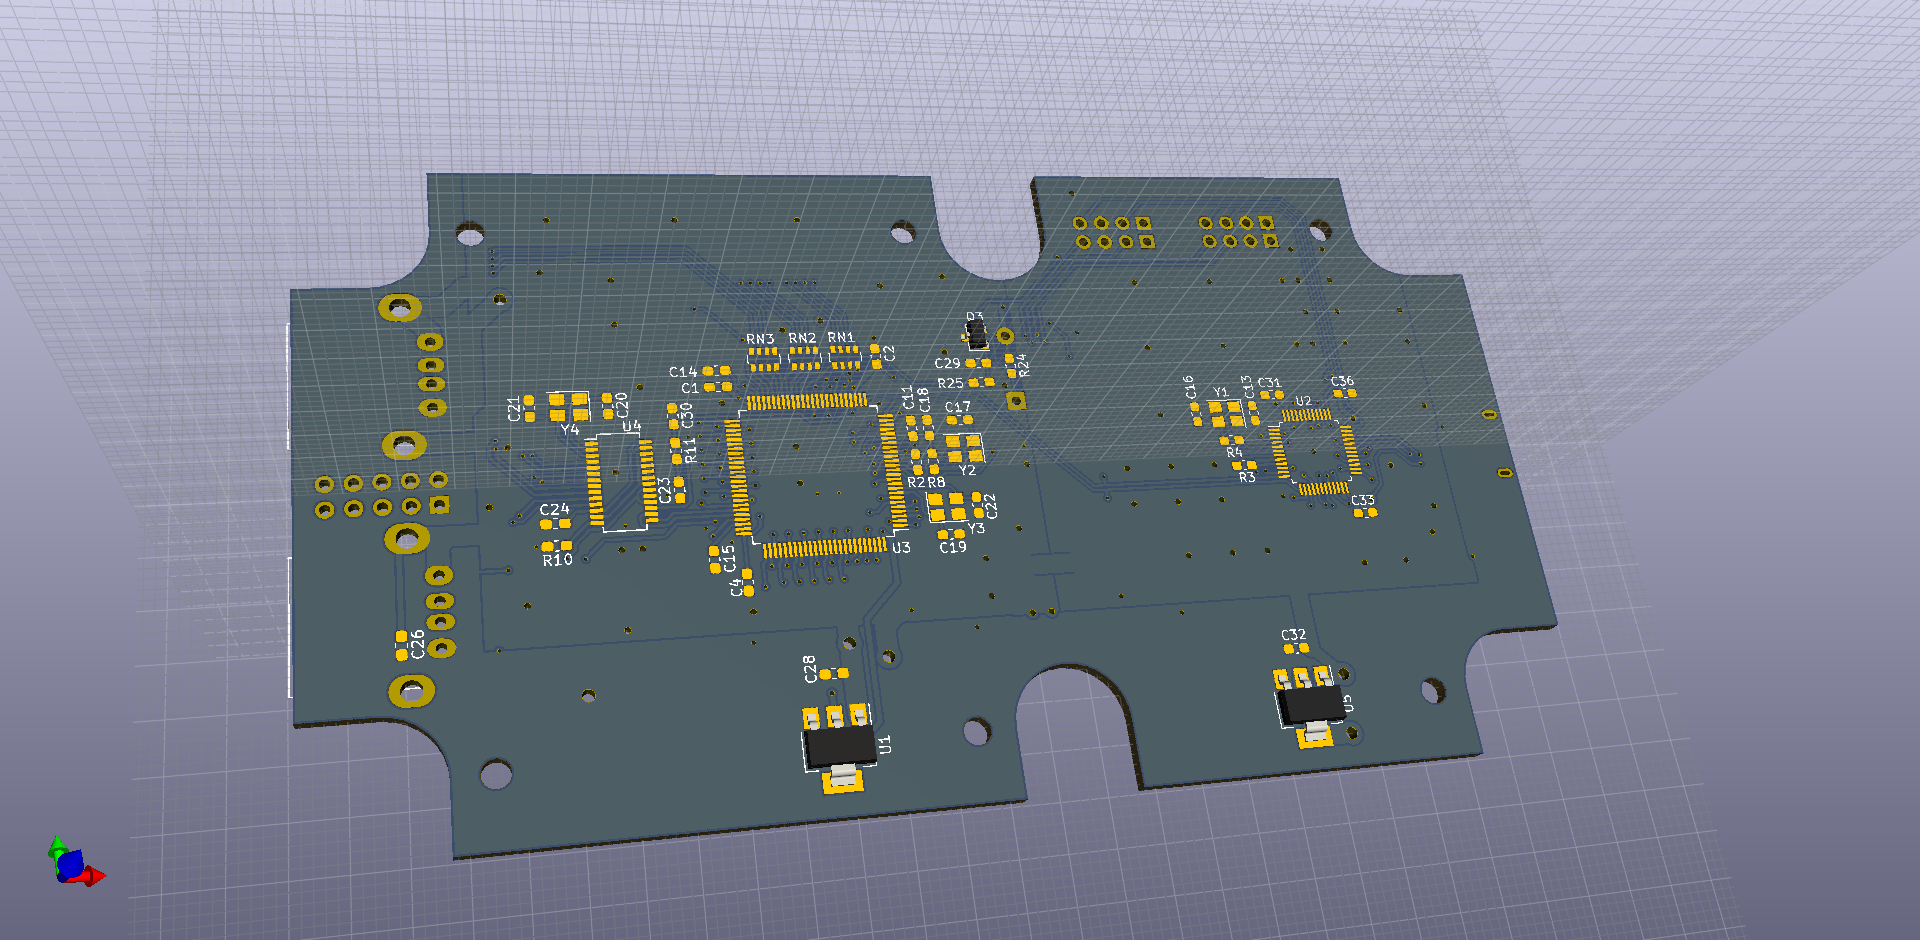
\includegraphics[width=0.8\textwidth]{pcb_front.png}
%        \caption{PCB front}
%    \end{subfigure} %
%    \begin{subfigure}[b]{0.8\textwidth}
%        \centering
%        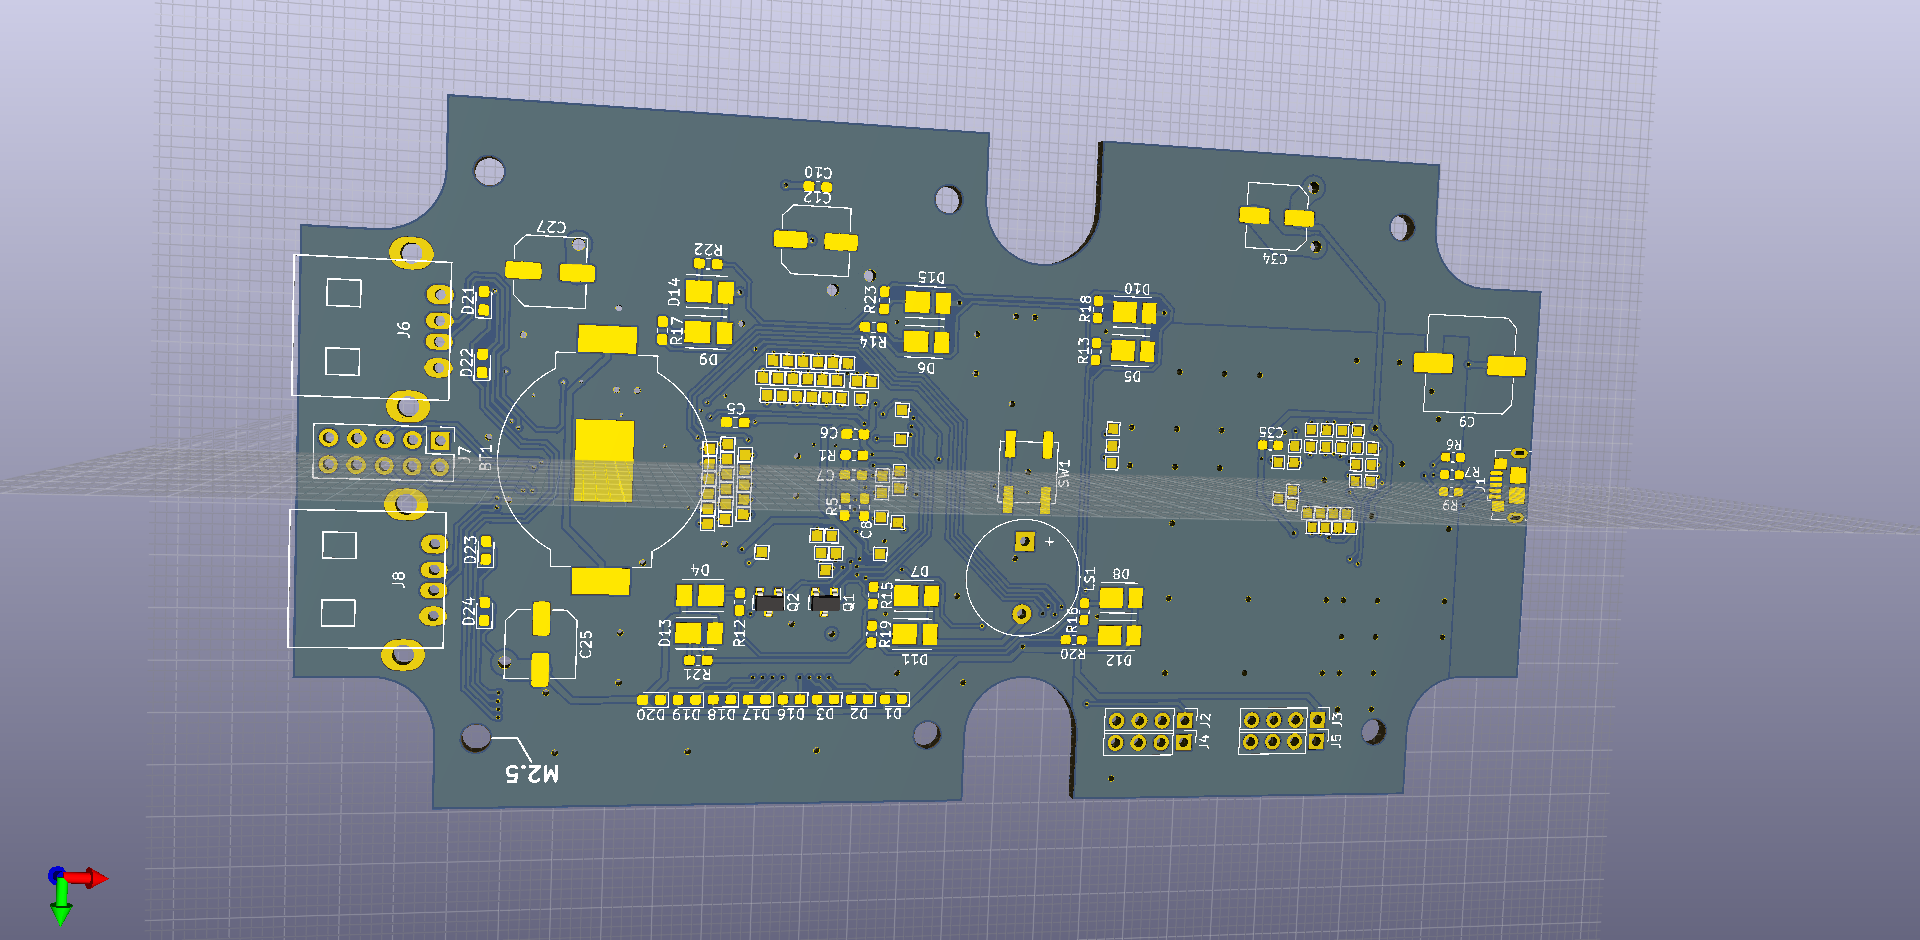
\includegraphics[width=0.8\textwidth]{pcb_back.png}
%        \caption{PCB back}
%    \end{subfigure}
%    \caption{PCB design 3D renderings}
%    \label{fig:pcb3d}
%\end{figure}
%
%\begin{figure}[H]
%    \centering
%    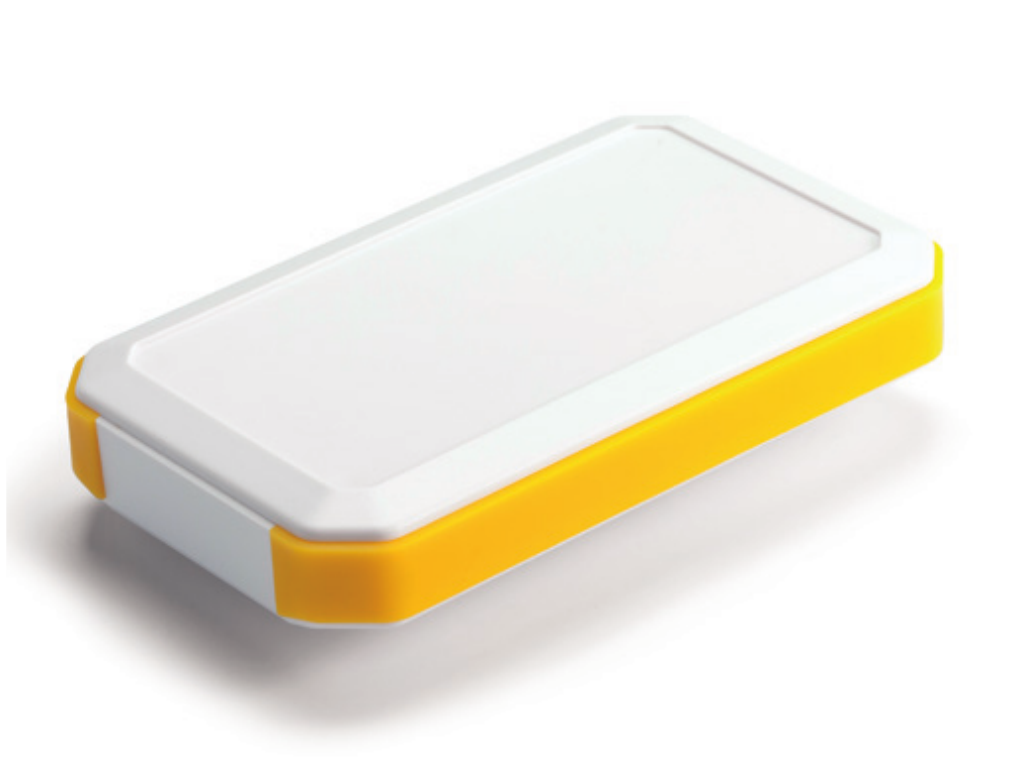
\includegraphics[width=0.6\textwidth]{takachi_case.png}
%    \caption{Off-the-shelf enclosure the PCB is made to fit}
%    \label{fig:case}
%\end{figure}

%\subsection{Attack surface in reasonably secure systems}
%\begin{figure}
%\tikzstyle{block} = [rectangle, draw, text centered, minimum height=4em]
%\begin{tikzpicture}[node distance=2cm, auto]
%   \node[block](matrix){Key matrix}
%   \node[block](hidctrl){Keyboard controller}
%   \node[block](hubs){USB hubs}
%   \node[block](roothub){USB host controller}
%   \node[block](pcie){PCIe bus}
%   \node[block](sys-usb-kernel){USB VM kernel}
%   \node[block](sys-usb-agent){USB VM userspace agent}
%   \node[block](dom0){dom0 agent}
%\end{tikzpicture}
%\label{qubes-hid-stack}
%\caption{The USB HID input stack in a QubesOS setup}
%\end{figure}

\nocite{*}
\printbibliography

\appendix
\section{Project state}
A working prototype has been completed.

\subsection{Completed}
\begin{itemize}
    \item Rough protocol design
    \item Protocol implementation based on \textcite{perrin01} using noise-c (microcontroller) and noiseprotocol (python/host)
    \item SRAM-based key storage with SRAM wear levelling
    \item host/device signature checking
    \item host/device key generation
    \item proper circuit design because I was bored last weekend (see appendix \ref{ch:renderings})
\end{itemize}

\subsection{Open issues}
\begin{itemize}
    \item Both noise-c and noiseprotocol have poor code and API quality. Since most noise functionality is not needed,
        just implement the protocol in bare C/python based on cryptographic primitives and scrap higher-level protocol
        implementations (though they've been useful so far during prototyping).
    \item Implement HID mouse host support
    \item Test USB hub support
    \item Replace the serial link with a custom USB link using an STM32F103 instead of the CH340G USB/serial converter
    \item Properly integrate prototype host client with qubes infrastructure
    \item Implement photodiode/monitor-based pairing side-channel
\end{itemize}

\section{Possible directions}
\begin{itemize}
    \item Elaborate handshake security properties
        \begin{itemize}
            \item Possibly investigate other applications of this type of interactive handshake
            \item Possibly contrast to carmera/other backchannel systems
%            \item IMHO the pairing scheme is the most interesting part of this project from a scientific point of view
% 			\item Prove security
        \end{itemize}
    \item Elaborate overall security properties of QubesOS-based system
    \item Elaborate possible DisplayPort/HDMI-based display encryption $\rightarrow$ Bunnie's NeTV2 w/ HDMI/eDP converter
    \item Elaborate possible encrypted remote input (SSH) setups
        \begin{itemize}
            \item This might turn out to be really interesting
            \item For this to be usable the host needs to tell the device at least which keyslot to use which could turn
                out to be complex to implement securely
            \item Considering complexity, this might turn into its own research project
        \end{itemize}
    \item Showcase secure hardware interface design, contrast with wireguard protocol design
        \begin{itemize}
            \item Formally derive handshake security properties
            \item Formally derive host/device protocol security properties using noise spec
            \item Formally verify and thouroughly unit-test the host/device protocol implementation on all layers
            \item IMHO this is the most interesting part of this project from an engineering point of view
        \end{itemize}
% Waiting
    \item Create custom hardware prototype
    \item Benchmark cryptography routines (will likely turn out to be ``wayyy fast'' for HID, fast enough for full-speed
        USB. High-speed cannot be done with the current architecture as we can't get data out the chip at high-speed
        data rates. \textcite{srivaths01} raise the issue of running crypto on embedded systems, but in this case it
        turns out with somewhat modern hardware and cryptography there is no problem at all.
\end{itemize}
\end{document}
